\chapter{力学与相对论}
正如绪论中所介绍的,力学(经典力学)研究的对象是物体的机械运动,更准确得说是研究若引力场中宏观物体的低速运动。
\begin{center}
\begin{align}
\text{\simhei{研究对象}:}& \text{\underline{宏观物体}在\underline{弱引力场}中\underline{低速运动}}  \notag \\
&\text{($\frac{GM}{rc^2}\ll1$时称为弱引力场,时空平直)} \notag \\
&\text{($\frac{v}{c}\ll1$时称为低速运动,伽利略、牛顿时空)}\notag \\
&\text{($\frac{H}{\bar{h}}\gg1$时称为宏观物体,物体运动状态可以用经典力学描述)}\notag
\end{align}
\end{center}

$H$为体系具有作用量的纲的“自然”动力学变量。前两个条件不满足我们必须用相对论(狭义相对论、广义相对论)来讨论,后一个条件不满足必须用量子力学来讨论。

我们将从最简单的质点讨论起,然后讨论质点为固体和流体等较为复杂的情况。

经典力学的内容包括运动学和动力学两个方面,运动学研究物体运动状态如何描述,以及描述运动状态的物理量之间的关系。而动力学研究物体运动状态的变化和物体与外界相互作用的关系。通常所说的力学规律之的主要是动力学规律。

力学规律的表述有几种不同的形式,用数学的语言来讨论,分别是:
\[
\begin{cases}
\text{不变分形式——牛顿形式(微分形式,积分形式)}\\
\text{变分形式(\A{variational form})}
	\begin{cases}
	\text{微分形式}\begin{cases}
		\text{拉格朗日力学(\A{Lagrangian mechanics})}\\
		\text{哈密顿力学(\A{Hamiltonian mechanics})}
		\end{cases}\\
	\text{积分形式——最小作用量原理(\A{Principle of least action})}
	\end{cases}
\end{cases}
\]

通常把力学规律的变分形式成为分析力学。分析力学的形式可以推广到物理学的其他领域,因而有着更普遍的意义。

本课程主要介绍牛顿形式、分析力学部分只做简略的介绍。

\section{质点运动的描述}
\subsection{质点、参考系、坐标系}
在物理学中为了研究方便,通常将研究的对象“理想化”,突出主要特征,忽略其次要因素,从而简化相应的物理模型以及相应的数学模型。力学中所谓的质点、刚体(有限自由度)、理想流体,完全弹性介质(以上为无线自由度)。热力学和统计物理学中所谓理想气体,电磁学中所谓点电荷、偶极子,理想导体都属于这样的模型。

以质点为例。

\subsubsection{质点}若我们考察的物体在所研究的问题中物体本身的大小和形状比之所考察的运动的线度小得多时,我们可以突出物体所具有的质量在所在空间中占有一定位置,这样两个因素用$(m,\vec{\gamma})$来描述,而忽略形状、大小和内部运动等次要因素。把物体视为具有质量而没有大小的对象。这就是所谓“质点”的概念。例如:当我们讨论地球绕太阳的公转运动时,我们把地球视为质点。而讨论地面上不同纬度处不同物体运动的差别时,我们必须把地球当作一个绕固定轴转动的刚体了。

要描述质点的运动首先要建立参考系、坐标系。
\subsubsection{参照系}

参照系的问题实际上是不同的观测者的问题。
\begin{description}
\item[参照空间]与参照物固连的三维空间;
\item[参照时间]与参照物固连的时钟所记录的时间;
\end{description}
参照空间与之固连的时钟组合称为参照系,通常用$S(O-XYZ),S'(O'-X'Y'Z')$来表示。在相对论的情况下,参照系表示为$S(O-ct,XYZ),S'(O'-ct',X'Y'Z')$。
\subsubsection{坐标系}
为定量地描述质点在参照系中的位置,而在参照空间中选定一组基矢(通常是正交的)以及相应的一组坐标,这样就可以用数学来表述空间中的矢量了。

对于三维的平直空间,常用的坐标系有:
\begin{description}
\item[直角坐标系]基矢为$(\vec{e_x},\vec{e_y},\vec{e_z})$或$(\vec{e_i},\vec{e_j},\vec{e_k})$,坐标记为$(x,y,z)$;
\item[平面极坐标]基矢为$(\vec{e_r},\vec{e_\varphi})$,$\vec{e_r},\vec{e_\varphi}$分别沿着$r,\varphi$增加的方向,随质点位置而变;
\item[球坐标系]基矢为$(\vec{e_r},\vec{e_\theta},\vec{e_\varphi})$,分别表示径、经度、纬度;
\item[柱坐标系]基矢为$(\vec{e_k},\vec{e_\varphi},\vec{e_z})$,对研究有对称的问题较方便;
\end{description}

\begin{figure} [ht]
\centering
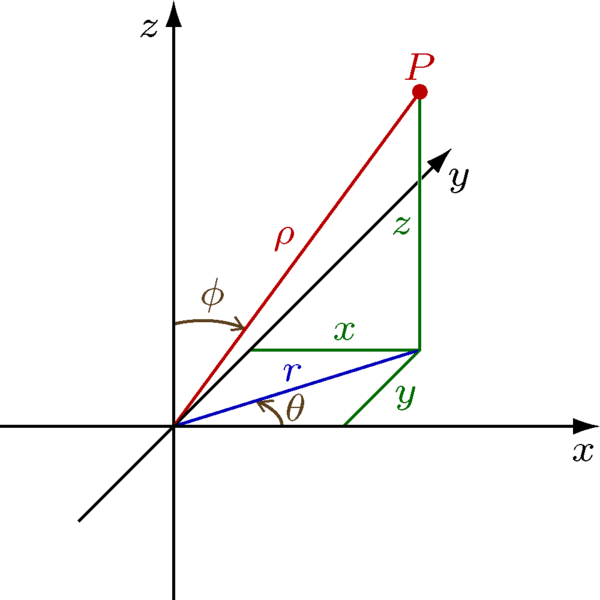
\includegraphics[scale=.35]{600px-Spherical_Coordinates.png}
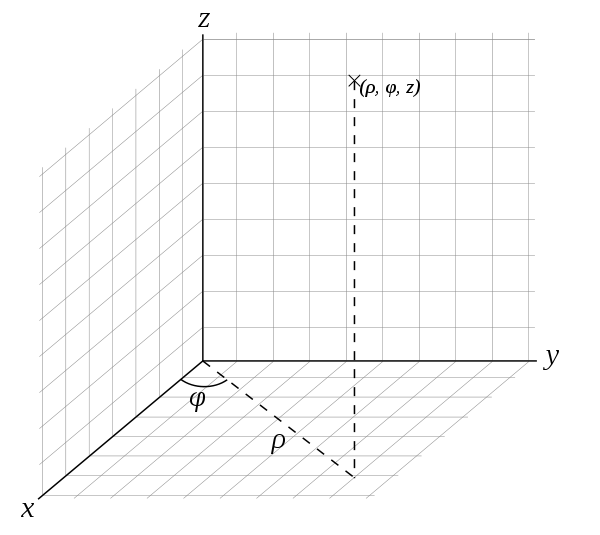
\includegraphics[scale=.4]{600px-Cylindrical_with_grid.svg.png}
\caption{\simsun 用球坐标系(左)和柱坐标系(右)表示三维空间内一个点的位置}
\label{600px-Cylindrical_with_grid.svg.png_600px-Spherical_Coordinates.png}
\end{figure}

此外还有一种自然坐标系(或本性坐标系),这是一种质点瞬时运动状态决定基矢的坐标系。其基矢为$\vec{e_\iota},\vec{e_n},\vec{e_\nu}$(或$\vec{c},\vec{n},\vec{b}$)分别表示该时钟质点运动的切向、主法向和次法向。

\subsection{质点运动的描述}
经典力学史研究物体的机械运动,所谓机械运动是物体空间位置随时间变动而变动的,物体在空间的位置要用矢量来描述,运动则用位置对事件变量$t$的依赖关系以及对时间的一次微商(速度),二次微商(加速度)等物理量来描述,因此要熟悉机械运动的描述,必须有关矢量和矢量的微分、积分运动。

我们还是首先将注意力集中在质点运动的描述上。

\subsubsection{位置矢量$\vec{\gamma}$}
$\vec{\gamma}$在各坐标系下的表示:\begin{description}
\item[直角坐标系]
	$\vec{\gamma}=x\vec{i}+y\vec{j}+z\vec{k}$,
	$\vec{\gamma}=(x,y,z)$
\item[极坐标系]
	$\vec{\gamma}=r\vec{e_r}$,$\vec{e_r}$再由$\varphi$决定,
	$\vec{\gamma}=(r,\varphi)$
\item[球坐标系]
	$\vec{\gamma}=r\vec{e_r}$,$\vec{e_r}$再由$\theta,\varphi$决定,
	$\vec{\gamma}=(r,\theta,\varphi)$
\item[柱坐标系]
	$\vec{\gamma}=\rho\vec{e_\rho}+z\vec{e_z}$,
	$\vec{e_\rho}$再由$\varphi$决定,
	$\vec{\gamma}=(\rho,\varphi,z)$
\end{description}


\subsubsection{速度矢量$\vec{v}$}\begin{description}
\item[定义(一维运动)]
$\vec{v}=\lim_{\varDelta t\to0}\frac{\varDelta x}{\varDelta t}=\frac{dx}{dt}$
\item[定义(三维空间)]
$\vec{v}=\frac{d\vec{r}}{t}=\lim_{\varDelta t\to0}\frac{\varDelta\vec{r}}{\varDelta t}$
\item[在直角坐标系下以分量表示]

\begin{align}
\vec{v}&=\frac{d\vec{r}}{t}=\frac{d}{dt}(x\vec{i}+y\vec{j}+z\vec{k}) \notag \\
&=\frac{dx}{dt}\vec{i}+x\frac{d\vec{i}}{dt}+\frac{dy}{dt}\vec{j}+y\frac{d\vec{j}}{dt}+\frac{dz}{dt}\vec{k}+z\frac{d\vec{k}}{dt} \notag \\
&=\frac{dx}{dt}\vec{i}+0+\frac{dy}{dt}\vec{j}+0+\frac{dz}{dt}\vec{k}+0=\dot{x}\vec{i}+\dot{y}\vec{j}+\dot{z}\vec{k} \notag
\end{align}

\item[在平面极坐标系下以分量表示]
\begin{align}
\vec{v} &= \frac{d\vec{\gamma}}{dt} = \frac{d}{dt}(r\vec{e_r}) =\frac{dr}{dt}\vec{e_r}+r\frac{d\vec{e_r}}{dt} \notag \\
&=\dot{r}\vec{e_r}+r\dot{\varphi}\vec{e_\varphi} =v_r\vec{e_r}+v_\varphi\vec{e_\varphi} \notag
\end{align}
\[\text{注意到其中}\frac{d\vec{e_r}}{dt} = \frac{d}{dt} (\cos\varphi \vec{i}+\sin\varphi\vec{j})=(-\vec{i}\sin\varphi+\vec{j}\cos\varphi)\frac{d\varphi}{dt} = \dot{\varphi}\vec{e_\varphi}\]
$v_r,v_\varphi$分别称作径向速度与切向速度。
\item[在球坐标系下以分量表示]
$\vec{v} = \dot{r} \vec{e_r} + r\,\dot\theta\,\vec{e_\theta} + r\,\dot\varphi\,\sin\theta \vec{e_\varphi} $
\end{description}

\subsubsection{加速度矢量$\vec{a}$}\begin{description}
\item[定义]$\vec{a}=\frac{d\vec{v}}{dt}$
\item[在直角坐标系下以分量表示]$\vec{a}=\ddot{x}\vec{i}+\ddot{y}\vec{j}+\ddot{z}\vec{k}$
\item[在平面极坐标系下以分量表示]
\begin{align}
\vec{a} &= \frac{d\vec{v}}{dt} =\frac{d(\dot{r}\vec{e_r}+r\dot{\varphi}\vec{e_\varphi})}{dt} =\ddot{r}\vec{e_r}+\dot{r}\frac{d\vec{e_r}}{dt}+\dot{r}\dot{\varphi}\vec{e_\varphi}+r\ddot{\varphi}\vec{e_\varphi}+r\dot{\varphi}\frac{d\vec{e_\varphi}}{dt} \notag \\
&=(\ddot{r}-\dot{r}\dot{\varphi}^2) \vec{e_r}+(2\dot{r}\dot{\varphi}+r\ddot{\varphi})\vec{e_\varphi} = a_r\vec{e_r}+a_\varphi\vec{e_\varphi} \notag
\end{align}
\[\text{注意到其中}\frac{d\vec{e_\varphi}}{dt} = \frac{d}{dt} (-\vec{i}\sin\varphi+\vec{j}\cos\varphi) = (-\vec{i}\cos\varphi-\vec{j}\sin\varphi)\frac{d\varphi}{dt}=-\dot\varphi\vec{e_r}\]
$a_r,a_\varphi$分别称作径向加速度与切向加速度。
\item[在球坐标系下以分量表示]
\begin{align}
\vec{a} = & \left( \ddot{r} - r\,\dot\theta^2 - r\,\dot\varphi^2\sin^2\theta \right)\vec{e_r} \notag \\
&+\left( r\,\ddot\theta + 2\dot{r}\,\dot\theta - r\,\dot\varphi^2\sin\theta\cos\theta \right) \vec{e_\theta} \notag \\
&+\left( r\ddot\varphi\,\sin\theta + 2\dot{r}\,\dot\varphi\,\sin\theta + 2 r\,\dot\theta\,\dot\varphi\,\cos\theta \right) \vec{e_\varphi}   \notag
\end{align}
\end{description}

\subsubsection{角速度矢量$\vec{\omega}$}
质点绕某一点转动时,常引入角速度矢量,常定义为$\vec{\omega}=\omega\vec{k}$,其中大小$\omega=\frac{d\varphi}{dt}$,方向$\vec{k}$由转轴方向的右手螺旋法则确定。

\begin{figure} [ht]
\centering
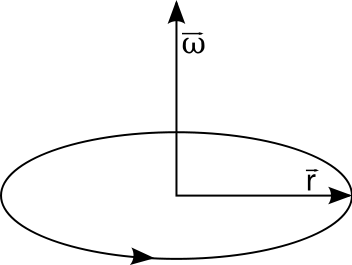
\includegraphics[scale=.35]{352px-Angular_velocity.svg.png}
\caption{$\vec{v}=\vec{\omega}\times\vec{r}$}
\label{352px-Angular_velocity.svg.png}
\end{figure}

后面我们可以看到刚体的运动可以分解为任意代表点的平动和绕该点的一个转动,因此描述刚体的运动常用到角速度矢量。

\section{参照系变换}
同一个物体的运动,在不同的参照系中观测,相应的运动学描述是不同的,但既然是同一物体的运动,不同参照系对他运动状态的描述——$\vec{r},\vec{v},\vec{a}$或$\vec{r}',\vec{v}',\vec{a}'$之间——是应该有联系的。了解他们之间的关系,对于分析许多现象是有帮助的。

例如我们常常需要比较:
\begin{center}
\begin{align}
\text{\simhei{例}:}& \text{地面参照系与地心参照系}  \notag \\
&\text{地球参照系与太阳参照系}\notag \\
&\text{实验室参照系与质心参照系} \notag
\end{align}
\end{center}



为叙述方便,在比较两个参照系时,指定某一参照系为静参照系(记作$S(O-XYZ)$),而另一个参照系为动参照系(记作$S'(O'-X'Y'Z')$)。在$S$系中观测到的运动指的是$(\vec{v},\vec{a})$称为\underline{绝对运动},而由$S'$系中观测到的运动称为\underline{相对运动},由$S'$相对于$S$运动而引起的\underline{附加速度$\vec{v_c}$}、\underline{附加加速度$\vec{a_c}$}称为牵连速度。应该指出,这里所谓的“静”与“动”,所谓“绝对”与“相对”,这些概念本来就不是绝对的,而是相对的。

必须指出,在经典力学中,认为不同参照系的时钟是相同的($t=t'$),即不同观测者所携带的时钟记录的时间是相对的($\varDelta t = \varDelta t'$),这是我们假设弱引力、低速运动的结果。

(相对论情况下为$S(O-tXYZ),S'(O'-X'Y'Z')$)
\subsection{$S'$系相对于$S$系作匀速直线运动}
\begin{align}
&\because \vec{\varDelta r} = \vec{\varDelta r'}+\vec{\varDelta R},\varDelta t = \varDelta t' \notag \\
&\therefore \frac{\vec{\varDelta r}}{\varDelta t} =\frac{\vec{\varDelta r'}}{\varDelta t}+\frac{\vec{\varDelta R}}{\varDelta t} \notag  \\
&\therefore \vec{v} =\vec{v'}+\vec{u} \notag
\end{align}
\begin{figure} [ht]
\centering
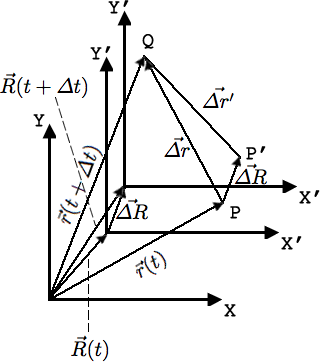
\includegraphics[scale=0.5]{frame_transform1.png}
\caption{\simsun 在$S$系中观测到的运动是从$P$到$Q$,在在$S'$系中观测到的运动则是从$P'$到$Q$}
\label{frame_transform1.png}
\end{figure}
\[ \frac{d\vec{u}}{dt}=0 \Rightarrow \vec{a}=\vec{a'} \]
\[
\text{结论:若$S'$相对$S$作匀速直线运动}
\begin{cases}
\vec{v}=\vec{v'}+\vec{u}\\
\vec{a}=\vec{a'}\\
\end{cases}
\]

\subsection{$S'$系相对于$S$系作任意方式平动}
设$\frac{d\vec{R}}{dt}=\vec{u},\frac{d\vec{u}}{t}=\vec{w}$,则类似地可得:
\[ \vec{v}=\vec{v'}+\vec{u}\quad \vec{a}=\vec{a'}+\vec{w}\]
\subsection{$S'$系相对于$S$系作匀角速度转动}
\begin{align}
&\because \vec{\varDelta r} = \vec{\varDelta r'}+\vec{\varDelta r_f},\varDelta t = \varDelta t' \notag \\
&\therefore \frac{\vec{\varDelta r}}{\varDelta t} =\frac{\vec{\varDelta r'}}{\varDelta t}+\frac{\vec{\varDelta r_f}}{\varDelta t} \notag  \\
&\therefore \vec{v} =\vec{v'}+\vec{\omega}\times\vec{r'} \notag
\end{align}

\begin{figure} [ht]
\centering
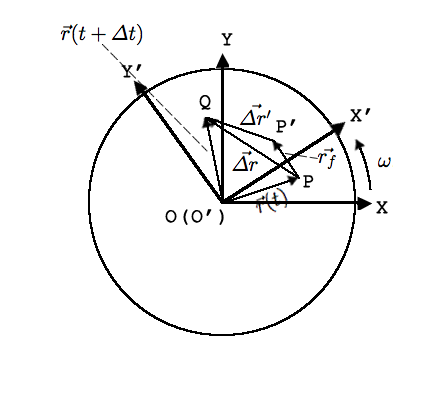
\includegraphics[scale=0.5]{frame_transform2.png}
\caption{\simsun 在$S$系中观测到的运动是从$P$到$Q$,在在$S'$系中观测到的运动则是从$P'$到$Q$}
\label{frame_transform2.png}
\end{figure}
\[\vec{a}=\frac{d\vec{v}}{dt}=\frac{d(\vec{v'}+\vec{\omega}\times\vec{r'})}{dt}=\frac{d\vec{v'}}{dt}+\frac{d(\vec{\omega}\times\vec{r'})}{dt}\]
\[\frac{d\vec{v'}}{dt}=\frac{d(\dot{x}\vec{i'}+\dot{y}\vec{j'}+\dot{z}\vec{k'})}{dt}=\ddot{x}\vec{i'}+\dot{x}\frac{d\vec{i'}}{dt}+\ddot{y}\vec{j'}+\dot{y}\frac{d\vec{j'}}{dt}+\ddot{z}\vec{k'}+\dot{z}\frac{d\vec{k'}}{dt}\]
\begin{align}
&\because \frac{d\vec{i'}}{dt}=\vec{\omega}\times\vec{i'},\ \frac{d\vec{j'}}{dt}=\vec{\omega}\times\vec{j'},\ \frac{d\vec{k'}}{dt}=\vec{\omega}\times\vec{k'} \notag \\
&\therefore \dot{x}\frac{d\vec{i'}}{dt}+\dot{y}\frac{d\vec{j'}}{dt}+\dot{z}\frac{d\vec{k'}}{dt} = \vec{\omega}\times(\dot{x}\vec{i'}+\dot{y}\vec{j'}+\dot{z}\vec{k'})= \vec{\omega}\times\vec{v'}\notag \\
&\therefore \frac{d\vec{v'}}{dt}=\vec{a'}+\vec{\omega}\times\vec{v'}\notag
\end{align}
\begin{align}
\frac{d(\vec{\omega}\times\vec{r'})}{dt} &= \vec{\omega}\times\frac{d\vec{r'}}{dt}=\vec{\omega}\times\frac{d(r_x\vec{i'}+r_y\vec{j'}+r_z\vec{k'})}{dt} \notag \\
&= \vec{\omega}\times(\dot{r_x}\vec{i'}+r_x\frac{d\vec{i'}}{dt}+\dot{r_y}\vec{j'}+r_y\frac{d\vec{j'}}{dt}+\dot{r_z}\vec{k'}+r_z\frac{d\vec{k'}}{dt}) \notag \\
&=  \vec{\omega}\times(\vec{v'}+r_x\omega\times\vec{i'}+r_y\omega\times\vec{j'}+r_z\omega\times\vec{k'}) \notag \\
&=  \vec{\omega}\times(\vec{v'}+\omega\times\vec{r'}) \notag \\
&=  \vec{\omega}\times\vec{v'}+ \vec{\omega}\times\vec{\omega}\times\vec{r'}\notag
\end{align}
\[
\therefore\vec{a}=\vec{a'}+\vec{\omega}\times(\vec{\omega}\times\vec{r'})+2\vec{\omega}\times\vec{v'} = \vec{a'} + \vec{a_l} + \vec{a_{col}}
\]
\[
\vec{a_l},\vec{a_{col}}\text{分别称作牵连加速度,科里奥利加速度(\A{Coriolis acceleration})}
\]
\subsection{$S'$系相对于$S$系作一般运动}
这里所指的一般运动,是指$O'$相对于$O$作任意运动,且$S'$系的坐标轴($O'-X'Y'Z'$)相对于$S$系的坐标轴($O-XYZ$)有转动,并且不一定是匀角速转动。

\begin{align}
\vec{v}&=\vec{v'}+\vec{v_{O'}}+\vec{\omega}\times\vec{r'} \notag \\
\vec{a}&=\vec{a'}+\vec{a_l}+\vec{a_{col}} \notag \\
\vec{a_l}&=\vec{a_0}+\dot{\vec{\omega}}\times\vec{r'}+\vec{\omega}\times(\vec{\omega}\times\vec{r}) \notag \\
\vec{a_{col}}&=2\vec{\omega}\times\vec{v'}\notag
\end{align}

由参照系变换可以推出以下结论:
\begin{enumerate}
\item 惯性系之间运动规律表述上的等价性
\item 在非惯性系中表述运动规律时出现惯性力的原因
\item 对于理解广义相对论中等效原理——惯性和引力等效,有一定启发意义
\end{enumerate}

